%\documentclass{article}
%\usepackage{graphicx,subfigure}
%\begin{document}

\begin{figure}[!h]
  \centering
  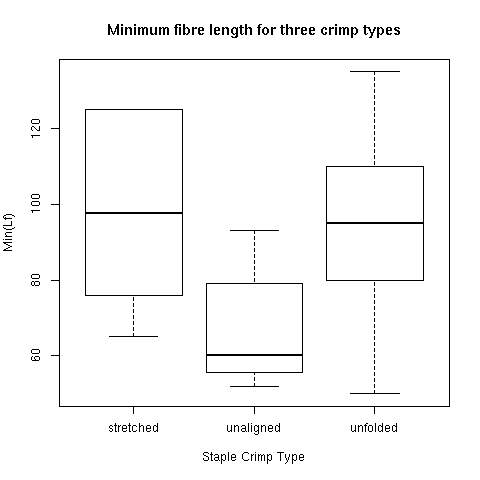
\includegraphics[width=1.1\textwidth]{figminlfbox.png}
%   minlfbox.png is original 
  \caption{Boxplot showing the minimum  fibre length for wools graded as {\em unaligned}, {\em stretched} and {\em unfolded} crimp types. Data from one Merino flock with 7,6, an d 9 sheep respectively representing each type}
  \label{fig:minlfbox}
\end{figure}

%\end{document}

